\documentclass[conference]{IEEEtran}

\usepackage{microtype}
\usepackage{graphicx}
\usepackage{cite}
\usepackage{float}
\usepackage{tikz}
\usetikzlibrary{arrows.meta,shapes.geometric}
\usepackage{url}
\usepackage{hyperref}

\hypersetup{
  colorlinks=true,
  linkcolor=black,
  citecolor=black,
  urlcolor=blue
}

\title{Learnwise: Design and Implementation of an Integrated Personalized Student Learning Platform}
\author{\IEEEauthorblockN{Jayanth Sri Sai, Vamsee Krishna, Meganadh, and Lohitha}
\IEEEauthorblockA{Department of Computer Science and Engineering\\
Koneru Lakshmaiah Education Foundation (KL University), India}}

\begin{document}
\maketitle

\begin{abstract}
Learnwise is a web application designed and implemented that integrates student assessment, progress monitoring, learning-resource recommendations, academic tutoring and teacher analytics. The application stores data of the quizzes, assignments, study time, and activities in a local SQLite database. A six aggregated features Random Forest classifier classifies the estimated learning level into one of three classes, Beginner, Intermediate, Advanced. A Rule Based component, based on the predicted level and subject performance, ranks incomplete resources. There are also course based quizzes and timed assessments, as well as class summaries and threshold alerts that teachers can access. The app is built using Streamlit, Pandas, Plotly and scikit-learn in Python. Being trained on synthetic examples whose labels are generated according to project defined rules, the internal test metrics of the classifier cannot ensure the performance on real learners. The software architecture and implementation is detailed in this paper and a plan for evaluation is proposed. Does not claim to measure learning gains.
\end{abstract}

\begin{IEEEkeywords}
personalized learning, educational recommender systems, learning analytics, student dashboards, machine learning
\end{IEEEkeywords}

\section{Introduction}
Pupils taking the same course may have different prior experience, assessment and study habits. Digital learning systems can offer the opportunity to organise information for learners and to identify content that might be pertinent to one person. The addition of personal features, however, does not mean an educational value. PLS reviews indicate that there are inconsistencies in the implementation and pedagogical results of PLS are not consistently reported in the literature \cite{zhang2020,dasilva2023}. Furthermore, according to a meta-analysis, effects observed are related to the educational context and the system design.

Learnwise is a capstone software prototype which integrates student and teacher focused study and teacher summary tools into a single application. Integrated implementation: Student activity is recorded and summarised, a broad-level estimate is made by a classifier, transparency rules rank learning resources and alert teachers, quizzes, exams and tutoring is made available via the same interface. The purpose of the system shall be to assist in review and study planning. Not validated for use as a diagnostic tool and not tested with regard to effectiveness in learning.

\section{Related Work}
The learner profile and learning-resource metadata have been used in educational recommender systems to select the content. In the systematic review of selected studies, da Silva et al. discovered that the evaluations of the recommender are typically technical, and that there is a lesser number of studies that focus on the pedagogical effectiveness of the recommender \cite{dasilva2023}. Zhang et al. aggregated 71 empirical studies on personalized-learning implementation and finding that there were variations in technology use and context, but that few studies were conducted on the whole-school outcomes of personalized learning \cite{zhang2020}. The results do support the idea that the logic used to make recommendations and the boundaries of its assessments should be made explicit in the report.

Learnwise does not employ collaborative filtering or learned recommendation model but rather a small size, rule based resource ranker. Adaptive hypermedia \cite{brusilovsky2001} is work that has been done earlier regarding user models and their usage to select and present the content. Learnwise has an explicit version of this idea limited to content selection and presentation. The student-level classifier is an ensemble of classifiers that is a Random Forest, a tree-based ensemble technique \cite{breiman2001}. Fine-grained knowledge-tracing systems combine the answers of different learners to compute an estimate of the state of the knowledge from a series of interactions with such systems as Bayesian models and recurrent neural models \cite{corbett1995,piech2015}. Learnwise uses six profile features that have been aggregated, and three broad classes. It is not in fact an intelligent tutoring or validated learner-modeling system, but rather a prototype that is a hybrid of profile-based classification with explicit recommendation rules.

On one hand, Learning Analytics (LA) and Educational Data Mining (EDM) are both concerned with describing and researching educational processes based on learner data, with at the same time posing questions regarding the scope, interpretation and privacy of the data \cite{siemens2013,romero2010}. Learning Analytics Dashboards are a summary of learner data that can be used for reflection and instructional decision making. Verbert et al. review the state of the art in dashboard applications for both learners and teachers, and suggest design and evaluation opportunities for both types of dashboard systems \cite{verbert2014}. Learnwise takes this concept of dashboard view by showing individual progress to students and aggregate signals to teachers, with a confirmation of the student views that are implemented in the screenshots in this paper.

Providing assessment and progress information that is clear and actionable can support learners to interpret what they are learning and plan what they need to do next. The importance of feedback, learner monitoring and goal-oriented feedback for adjustment have been discussed in the research on formative feedback and SLL literature \cite{shute2008,hattie2007,nicol2006,zimmerman2002}. Learnwise provides scores, weak-subject alerts, study goals and study achievements, without using a validated feedback intervention. Likewise, the tutor is a very simple question-answer dialogue system, while an intelligent tutoring system can employ a more complex learner model and data-driven instructional policies \cite{koedinger2013}.

\section{Requirements and System Architecture}
In this section, the requirements and system architecture are discussed.The requirements and system architecture are discussed.
The design has two roles. Students require a perspective on performance, course content, reporting and feedback on assessment, and a study aid. There should be a summary of the class and a means for teachers to see each student's record. The implementation is a single Python application, on a per-role basis. It is comprised of its main components (shown in Fig.~\ref{fig:architecture}).

\begin{figure*}[!t]
\centering
\resizebox{\textwidth}{!}{%
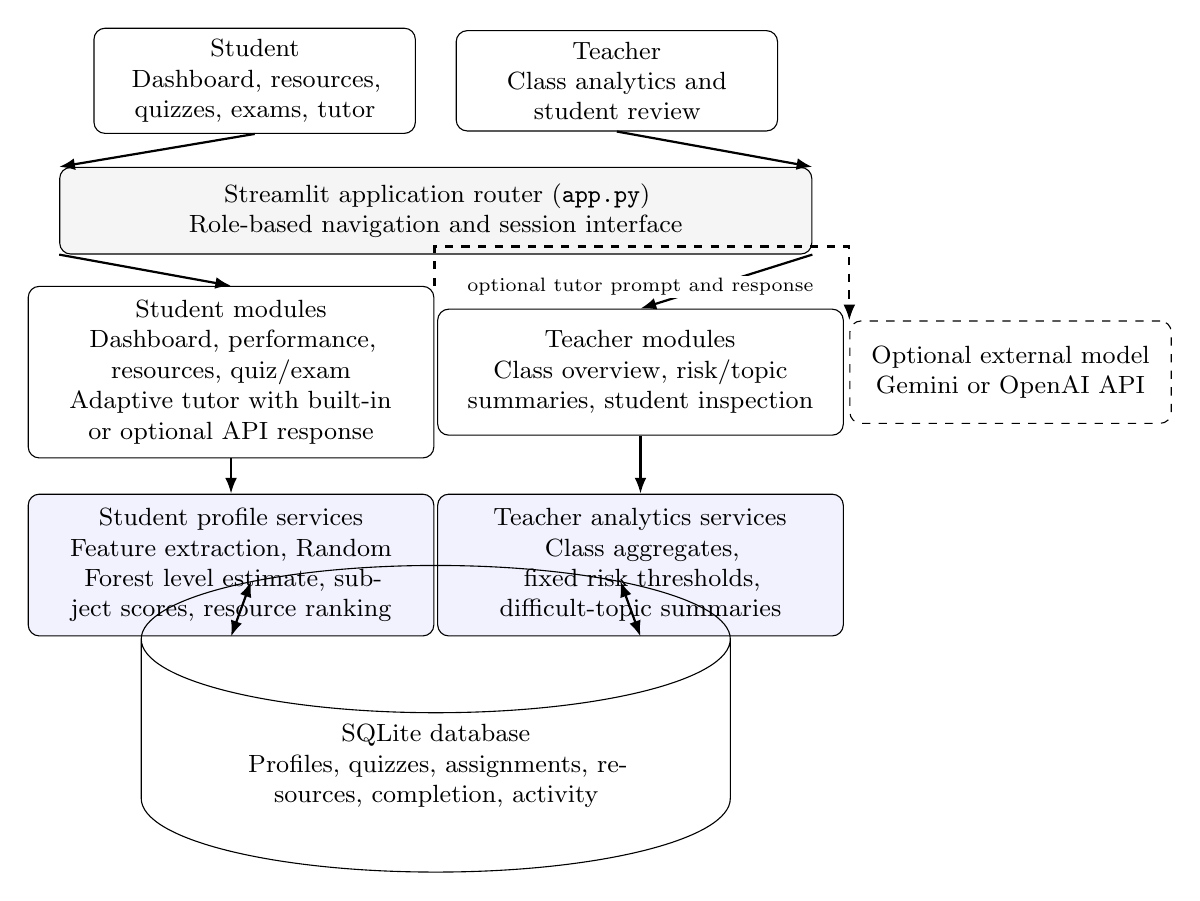
\begin{tikzpicture}[
  font=\small,
  userbox/.style={draw, rounded corners, align=center, text width=38mm, minimum height=10mm, inner sep=4pt},
  appbox/.style={draw, rounded corners, align=center, text width=92mm, minimum height=11mm, inner sep=5pt, fill=gray!8},
  module/.style={draw, rounded corners, align=center, text width=48mm, minimum height=16mm, inner sep=5pt},
  service/.style={draw, rounded corners, align=center, text width=48mm, minimum height=18mm, inner sep=5pt, fill=blue!5},
  store/.style={draw, cylinder, shape border rotate=90, aspect=0.25, align=center, text width=72mm, minimum height=15mm, inner sep=4pt},
  external/.style={draw, dashed, rounded corners, align=center, text width=38mm, minimum height=13mm, inner sep=4pt},
  flow/.style={-{Latex[length=2mm]}, thick},
  dataflow/.style={{Latex[length=2mm]}-{Latex[length=2mm]}, thick}
]
\node[userbox] (student) at (2.2,0) {Student\\Dashboard, resources, quizzes, exams, tutor};
\node[userbox] (teacher) at (6.8,0) {Teacher\\Class analytics and student review};
\node[appbox] (router) at (4.5,-1.65) {Streamlit application router (\texttt{app.py})\\Role-based navigation and session interface};
\node[module] (studentui) at (1.9,-3.7) {Student modules\\Dashboard, performance, resources, quiz/exam\\Adaptive tutor with built-in or optional API response};
\node[module] (teacherui) at (7.1,-3.7) {Teacher modules\\Class overview, risk/topic summaries, student inspection};
\node[service] (profile) at (1.9,-6.15) {Student profile services\\Feature extraction, Random Forest level estimate, subject scores, resource ranking};
\node[service] (analytics) at (7.1,-6.15) {Teacher analytics services\\Class aggregates, fixed risk thresholds, difficult-topic summaries};
\node[store] (database) at (4.5,-8.7) {SQLite database\\Profiles, quizzes, assignments, resources, completion, activity};
\node[external] (llm) at (11.8,-3.7) {Optional external model\\Gemini or OpenAI API};

\draw[flow] (student.south) -- (router.north west);
\draw[flow] (teacher.south) -- (router.north east);
\draw[flow] (router.south west) -- (studentui.north);
\draw[flow] (router.south east) -- (teacherui.north);
\draw[flow] (studentui.south) -- (profile.north);
\draw[flow] (teacherui.south) -- (analytics.north);
\draw[dataflow] (profile.south) -- (database.north west);
\draw[dataflow] (analytics.south) -- (database.north east);
\draw[flow,dashed] (studentui.north east) -- ++(0,5mm) -| (llm.north west);
\node[font=\scriptsize,fill=white,inner sep=1pt] at (7.1,-2.62) {optional tutor prompt and response};
\end{tikzpicture}%
}
\caption{Learnwise architecture. The application modules read and write student data through SQLite. The external language-model connection is optional; the tutor has a built-in response path.}
\label{fig:architecture}
\end{figure*}

\subsection{Data Model and Processing Flow}
There are tables for users, student profiles, subjects, quiz results, assignments, learning resources, completion progress, and learning activities, all of which are part of the database schema. A record of the quiz contains the following information: Course Subject, Topic, Score, Number of Questions, Number of Attempts, and Date. Helper functions are used to fetch the pertinent records on a dashboard or request for a recommendation, and then they are combined together with Pandas. The new record is added to SQLite when the quiz is submitted, and the profile prediction and dashboard summaries can then be formed from this record.

This system calculates an average mark for the subjects based on the marks from the quizzes and assignments. A score of less than 50\% indicates a weak subject, while a score of 75\% or more indicates strong subject. The difficulty level of an exam is saved to the label of the topic when creating a new timed exam, which enables you to report on the exam by topic and difficulty. Older quiz topics that do not have difficulty labels are not retroactively given a level.
\section{Implementation}
\subsection{Application and Persistence}
The user interface of the application has been coded using Streamlit, which supplies the dashboard, form, navigation, and chart elements of the application \cite{streamlit}. The entry point creates the database and sends a signed in user to student or teacher modules. There are Python modules handling authentication, database access, machine-learning inference, quizzes, recommendations, tutoring and analytics. SQLite offers local relational persistence in form of a database file \cite{sqlite}. A limitation on reproducibility is that the requirements do not state exact versions of the packages that need to be installed, but only minimum versions of Streamlit, Pandas, NumPy, scikit-learn, Plotly, Joblib, Requests, and Python-dotenv.

\subsection{Student-Level Classification}
The feature extractor creates 6 values: Mean quiz score, Mean assignment score, Log study time, Mean quiz attempts, Completed-resource count, Composite score (Mean quiz score + Mean assignment score - Log study time - Mean quiz attempts - Completed-resource count).
\[
S_{\mathrm{composite}} = 0.6S_{\mathrm{quiz}} + 0.4S_{\mathrm{assignment}}.
\]   
   
If records are missing, the application provides default values to complete the feature vector that is numeric. The model is trained with the scikit-learn \texttt{RandomForestClassifier}\cite{sklearnrf} class.

The training script mimics \(400\) records and partitions them into \(75\%/25\%\) training/validation sets. It uses a fixed random seed, balanced class weights, and trains \(100\) trees with a maximum depth of \(8\). There are heuristic conditions to determine synthetic labels: a composite score \(< 55\), study time \(< 8\) hours, and mean attempts \(> 3.5\) result in \textit{Beginner}; a composite score \(> 78\), study time \(\geq 14\) hours, and mean attempts \(\leq 2\) result in \textit{Advanced}; any other combination is classified as \textit{Intermediate}. The feature vector includes completed activities, but this feature is not directly incorporated into the label-generation conditions. The model is fitted and serialized using Joblib to obtain a model file. When a student identifier is provided, the predicted level is written to the corresponding student record. During inference, the predicted class is returned along with the associated model probabilities.

The repeated steps mean that this implementation can be repeated, but the examples held out have the same synthetic generation and labeling processes. The accuracy of these labels would reflect the success of recovery of the heuristic rules, not validity for educational placement. Therefore, no results of classifier accuracy are provided as a real world result for this reason.

Resource Ranking and teacher rules
The resource ranker will eliminate completed resources and then give them a relevance score. The individual who matched the resource gets 50 points. An adjacent-level match (Beginner/Intermediate) will earn a team 15 points, while a match between the difficulty of the resources and the predicted level will earn a team 30 points. If a video, quiz or practice-question resource is provided in a weak subject, it is worth an additional 20 points. Six top scoring resources are returned. This is a determinate heuristic which is not based on learner to resource interaction training nor on relevance judgments.

The teacher alerts are also based on a set of rules. A student is added to Needs Improvement list when their Average Quiz Score is less than 60\%, and they have one or more of the following conditions: Average Quiz Score is below 50\%, i.e., they have studied fewer than 50 minutes on average for each quiz, Logged Study Time is below 8 hours, or they have 2 or more subjects with poor score or 15 or more subject errors or they have 3 or more attempts on average to each quiz. Topic summaries present class quiz results in groups by subject and topic, and target the groups where the numbers of students that fail to get 60\% or above are at least 40\%. These are indicators that can be used by teachers to review but do not constitute a diagnosis.

\subsection{Assessment and Tutor}
Course and difficulty grouped practice questions. Timed exams will have a 30 minute time limit, save selected answers during the application session, and store the final score and the level of difficulty with the quiz score. Requests the full screen mode and reports tab changes or exits to full screen mode from the browser component. Two warnings will be issued; if you get a third one, you will be submitting your saved answers! No video, audio or screen capture is made.

The tutor firstly identifies the levels and areas of weakness predicted for the student. When the student sets up a Gemini or OpenAI key, the app sends a prompt to the service that consists of the student's level, weak-subject names, and question. If an API response is not available, then the built-in responder supplies hand-written topic-specific information for select computing concepts. It has a general fall-back of template based, which results in limited coverage and the quality of the answers. An external model may provide false feedback, a teacher or source of the course should be available to verify. Additionally, due to the optional API path, deployments should specify what prompt information is sent to the provider and be careful to apply adequate privacy controls \cite{pardo2014,unesco}.
\section{Results}
The following results present the interface that was implemented to be accessed by the students and the provided functions. They are not learning outcomes, but rather the software outcomes of a description.

\subsection{Dashboard and Subject-Level Performance}
The dashboard overview in Fig.~\ref{fig:dashboard-overview} presents progress indicators such as learning XP, streak, and quiz average.

\begin{figure}[H]
\centering
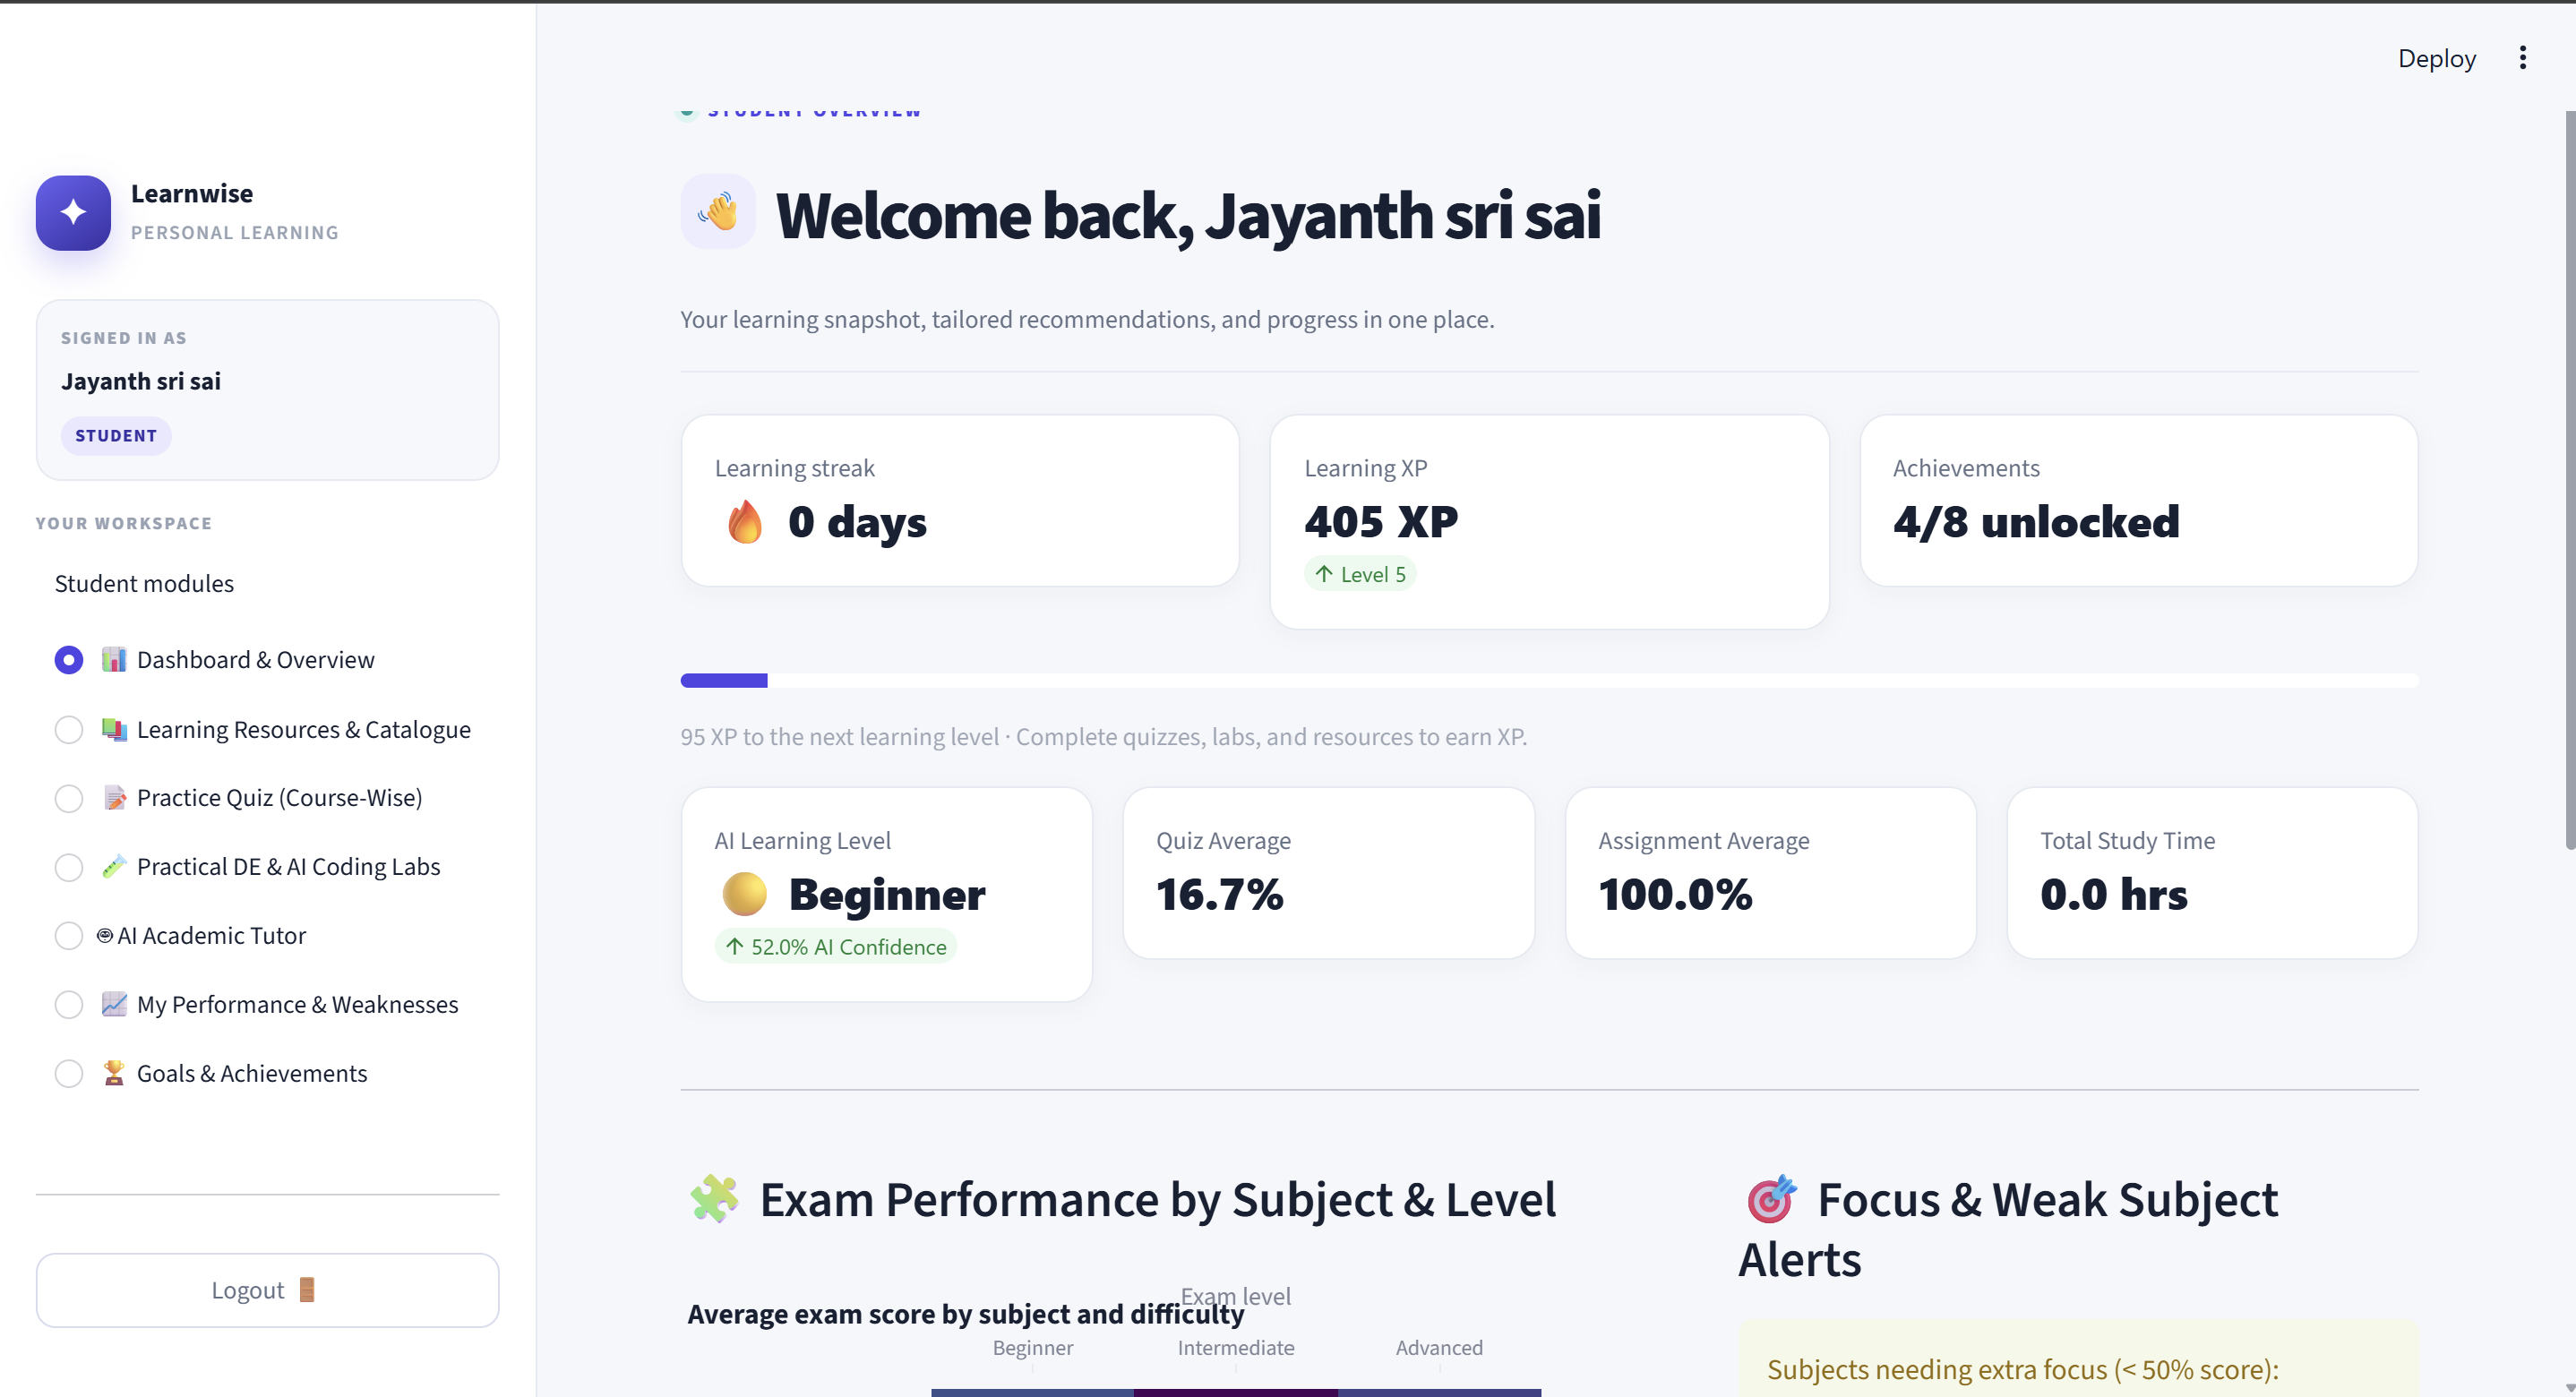
\includegraphics[width=\linewidth,height=1.8in,keepaspectratio]{figures/dashboard-overview.png}
\caption{Student overview and progress indicators. Values belong to the supplied demo account.}
\label{fig:dashboard-overview}
\end{figure}

Subject performance view Fig.~\ref{fig:dashboard-exam-performance}  contains a comparison of the average exam scores of subject and Beginner, Intermediate and Advanced. When a student's performance is below the set standard, the Focus alerts will identify this. This will enable the student to get an opportunity to remember sections that will require further practice.

\begin{figure}[H]
\centering
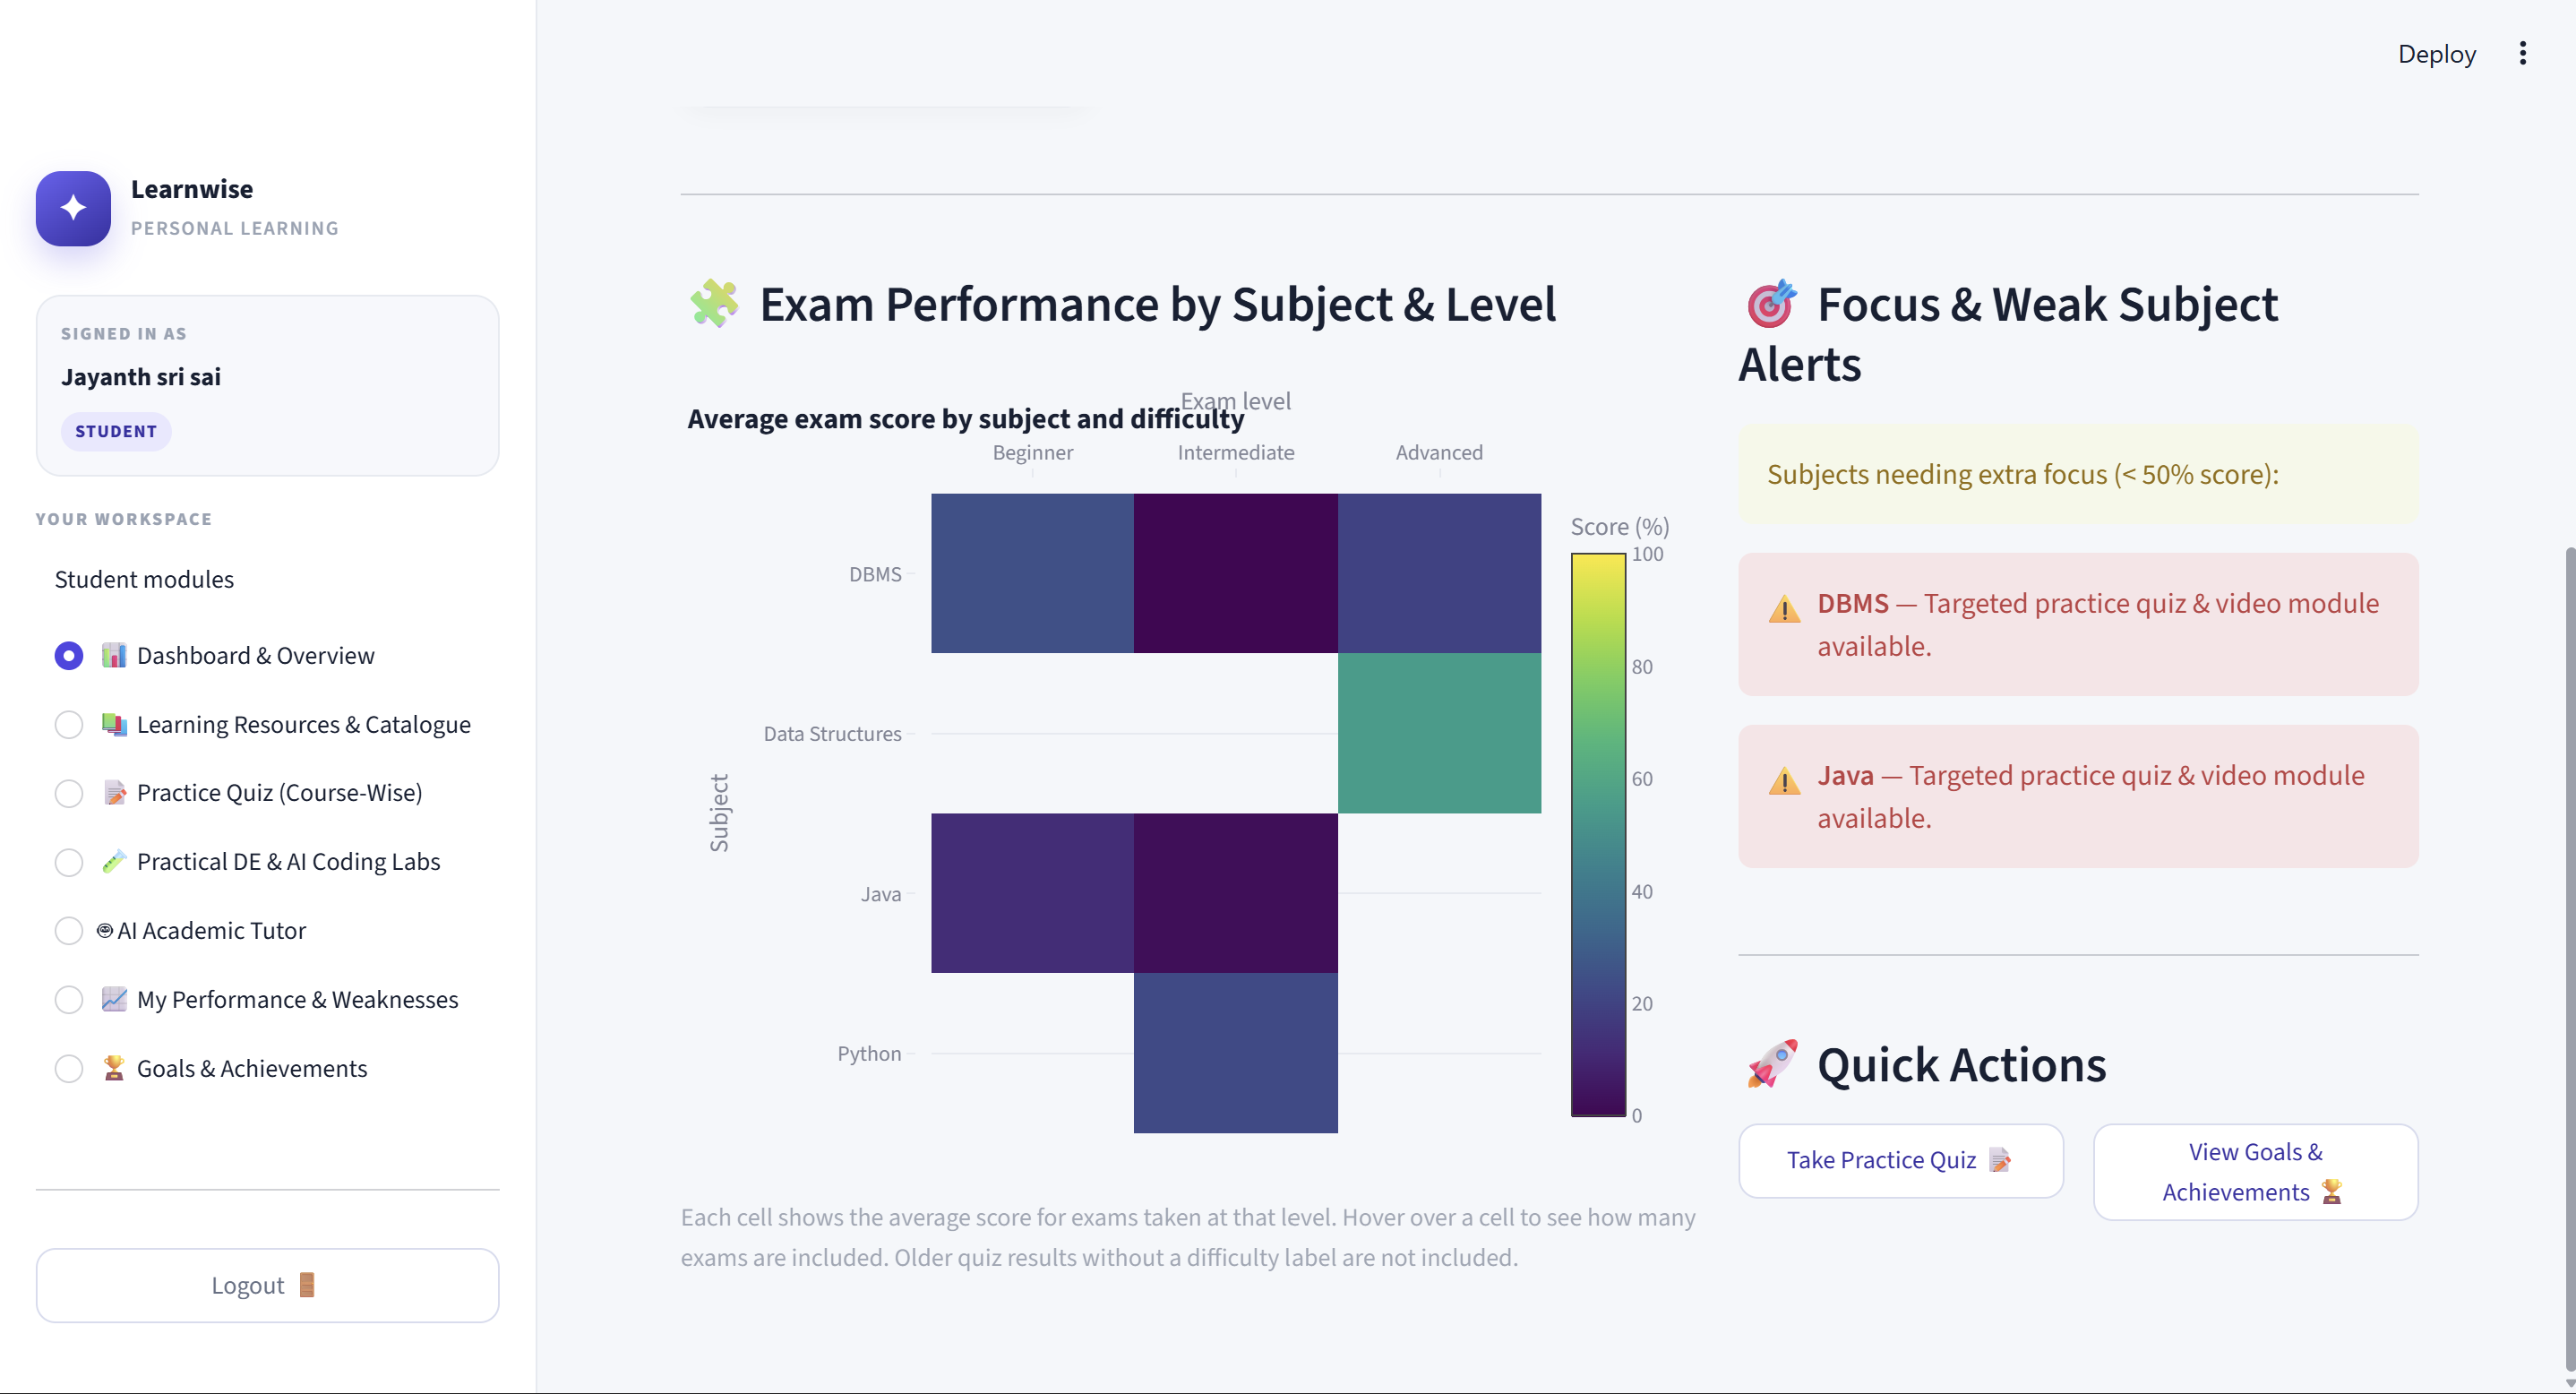
\includegraphics[width=\linewidth,height=1.8in,keepaspectratio]{figures/dashboard-exam-performance.png}
\caption{Subject scores by exam difficulty and focus alerts.}
\label{fig:dashboard-exam-performance}
\end{figure}

\subsection{Timed Exam and Tutor Workspace}
The student is able to choose a course, select a level of difficulty and then proceed to take the exam in a full-screen, timed session from the exam page. The policy for the setup time and two warnings – 30 minutes is displayed in Figure~\ref{fig:course-exam-setup}. The only screen shot that will be shown is the set up screen, NOT the answers or a grade for the exam.

\begin{figure}[H]
\centering
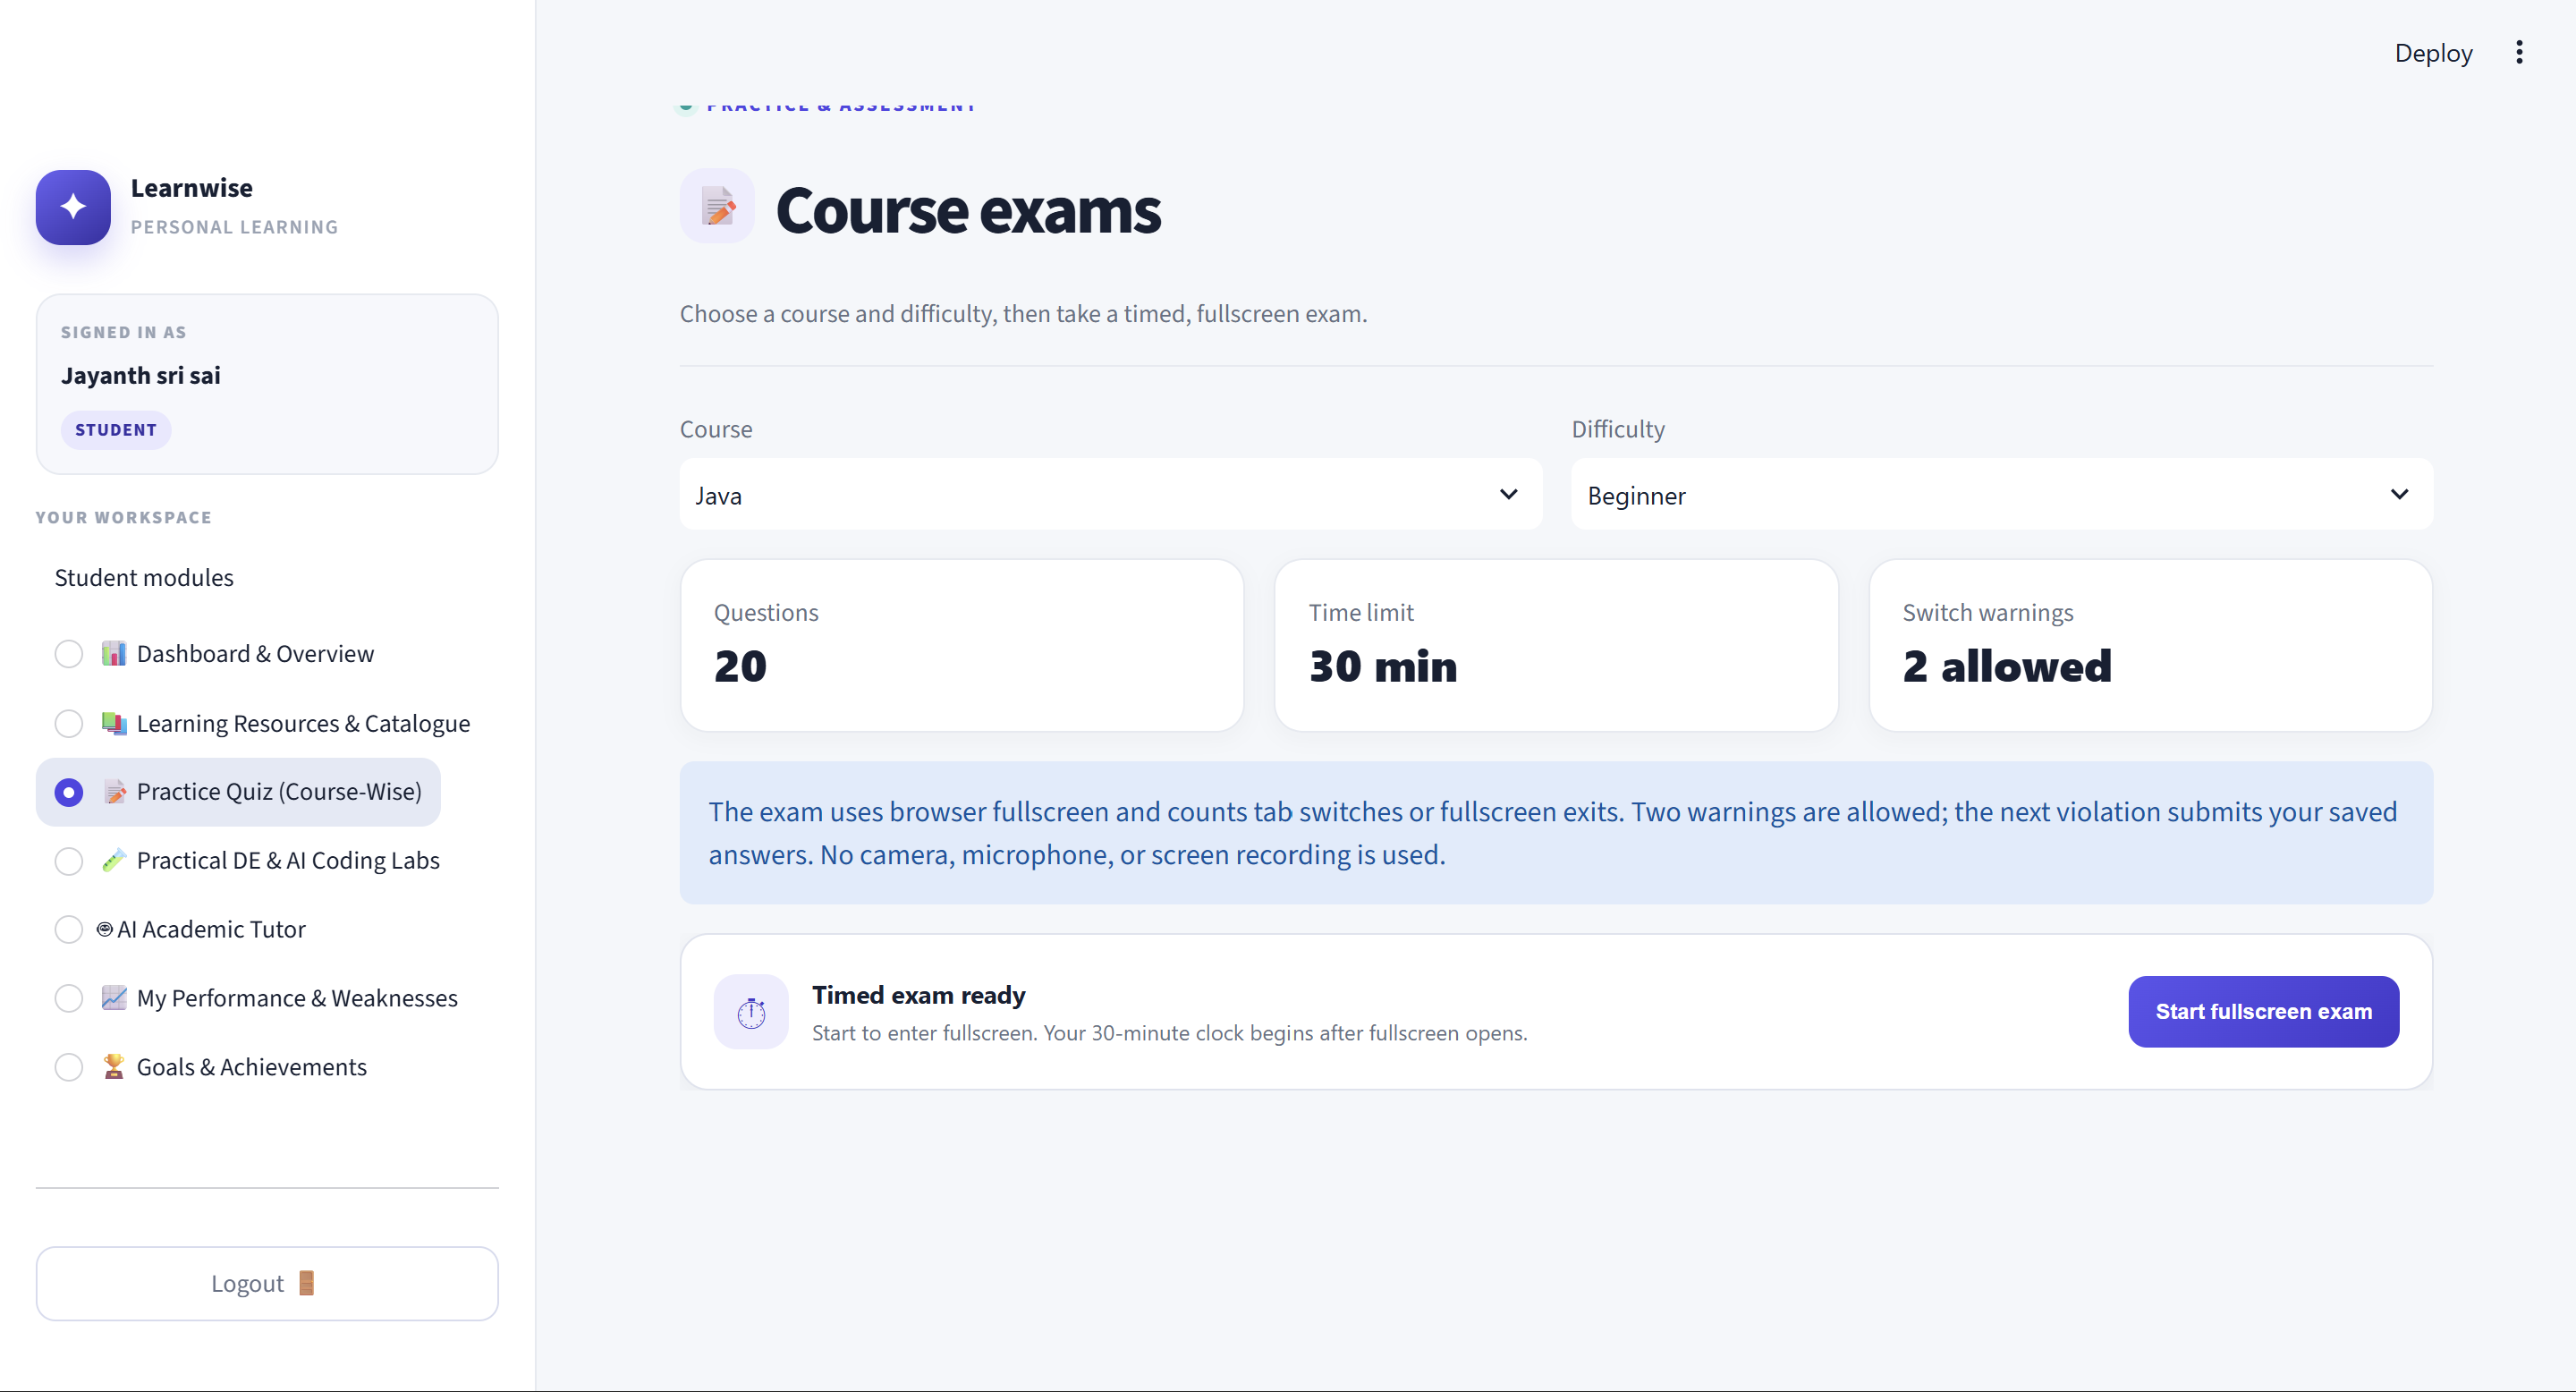
\includegraphics[width=\linewidth,height=1.8in,keepaspectratio]{figures/course-exam-setup.png}
\caption{Course exam setup, duration, and switch-warning policy.}
\label{fig:course-exam-setup}
\end{figure}

The tutor workspace in Fig.~\ref{fig:ai-academic-tutor} provides suggested question prompts and an input area for student questions.

\begin{figure}[H]
\centering
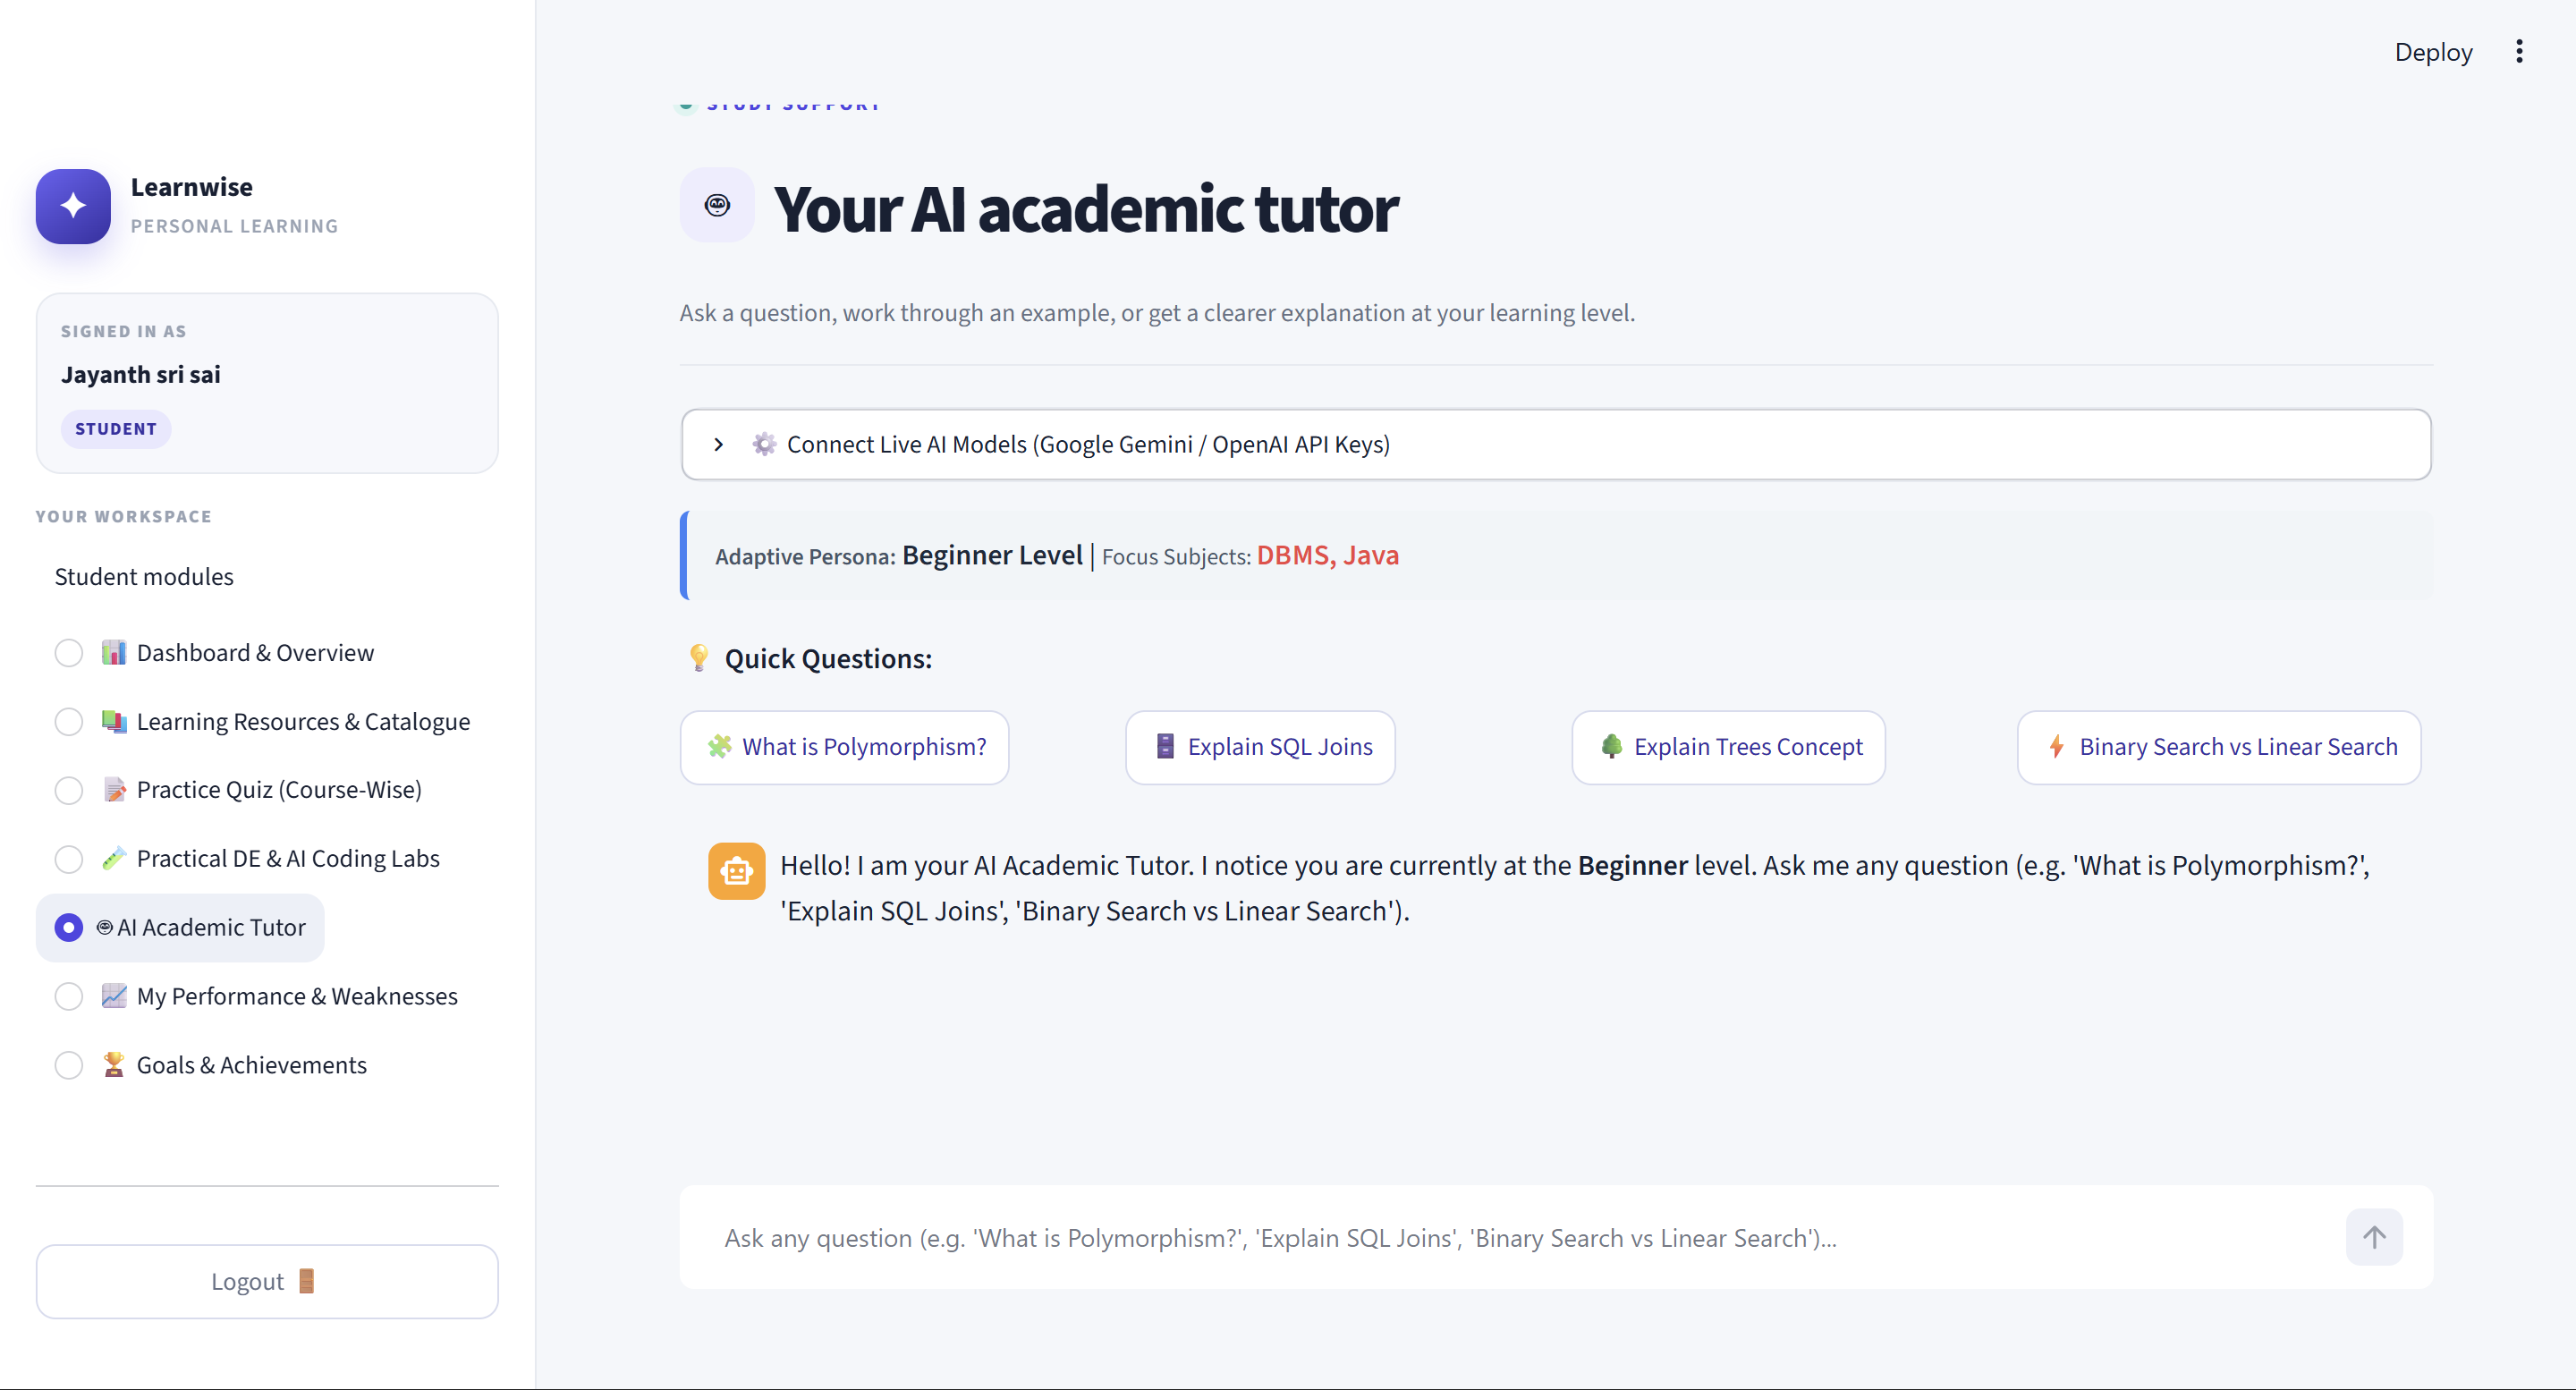
\includegraphics[width=\linewidth,height=1.8in,keepaspectratio]{figures/ai-academic-tutor.png}
\caption{Tutor workspace with quick-question prompts.}
\label{fig:ai-academic-tutor}
\end{figure}

\subsection{Performance Analytics and Goals}

The analytics page contains skill radar and domain level indicators. A figure of merit (fom) would be displayed in figure~\ref{fig:performance-analytics} as would be the radar.

\begin{figure}[H]
\centering
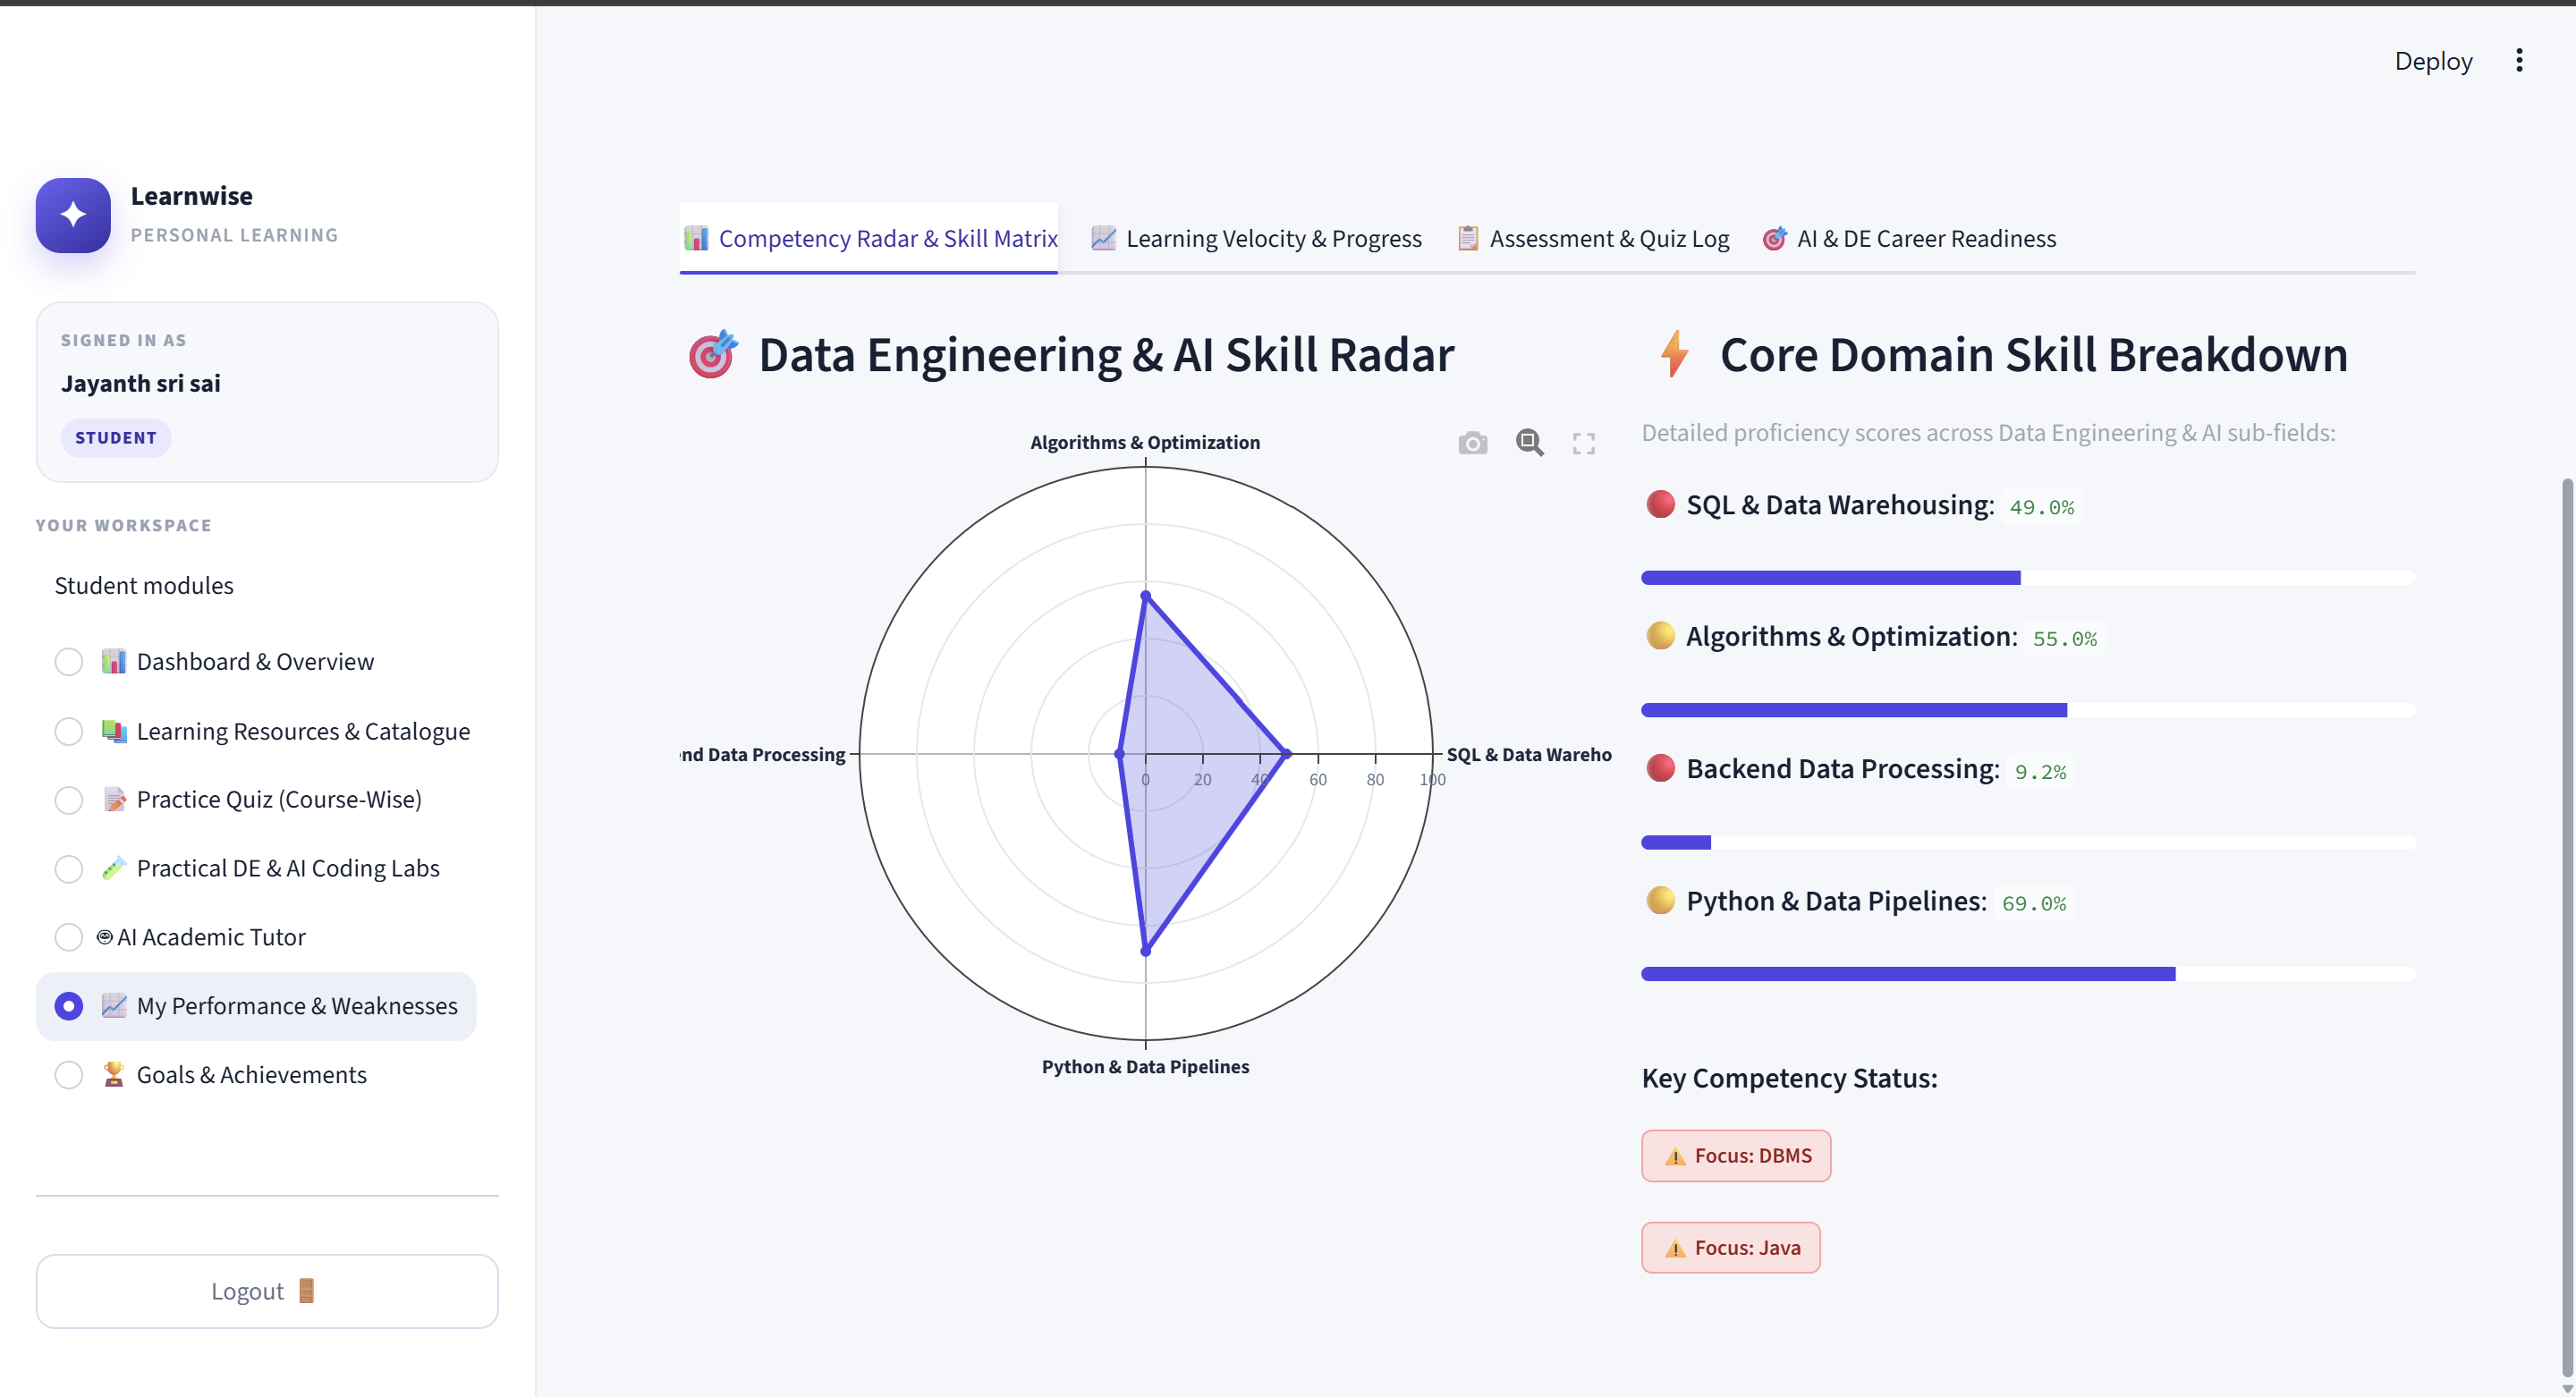
\includegraphics[width=\linewidth,height=1.8in,keepaspectratio]{figures/performance-analytics.png}
\caption{Skill radar and domain-level performance indicators.}
\label{fig:performance-analytics}
\end{figure}


The goals page (Fig.~\ref{fig:goals-achievements}) lists a summary of activity, learning streak and earned badges. The results displayed in the application are based on the ability to report the results and do not signify higher abilities or a higher score in the real world.

\begin{figure}[H]
\centering
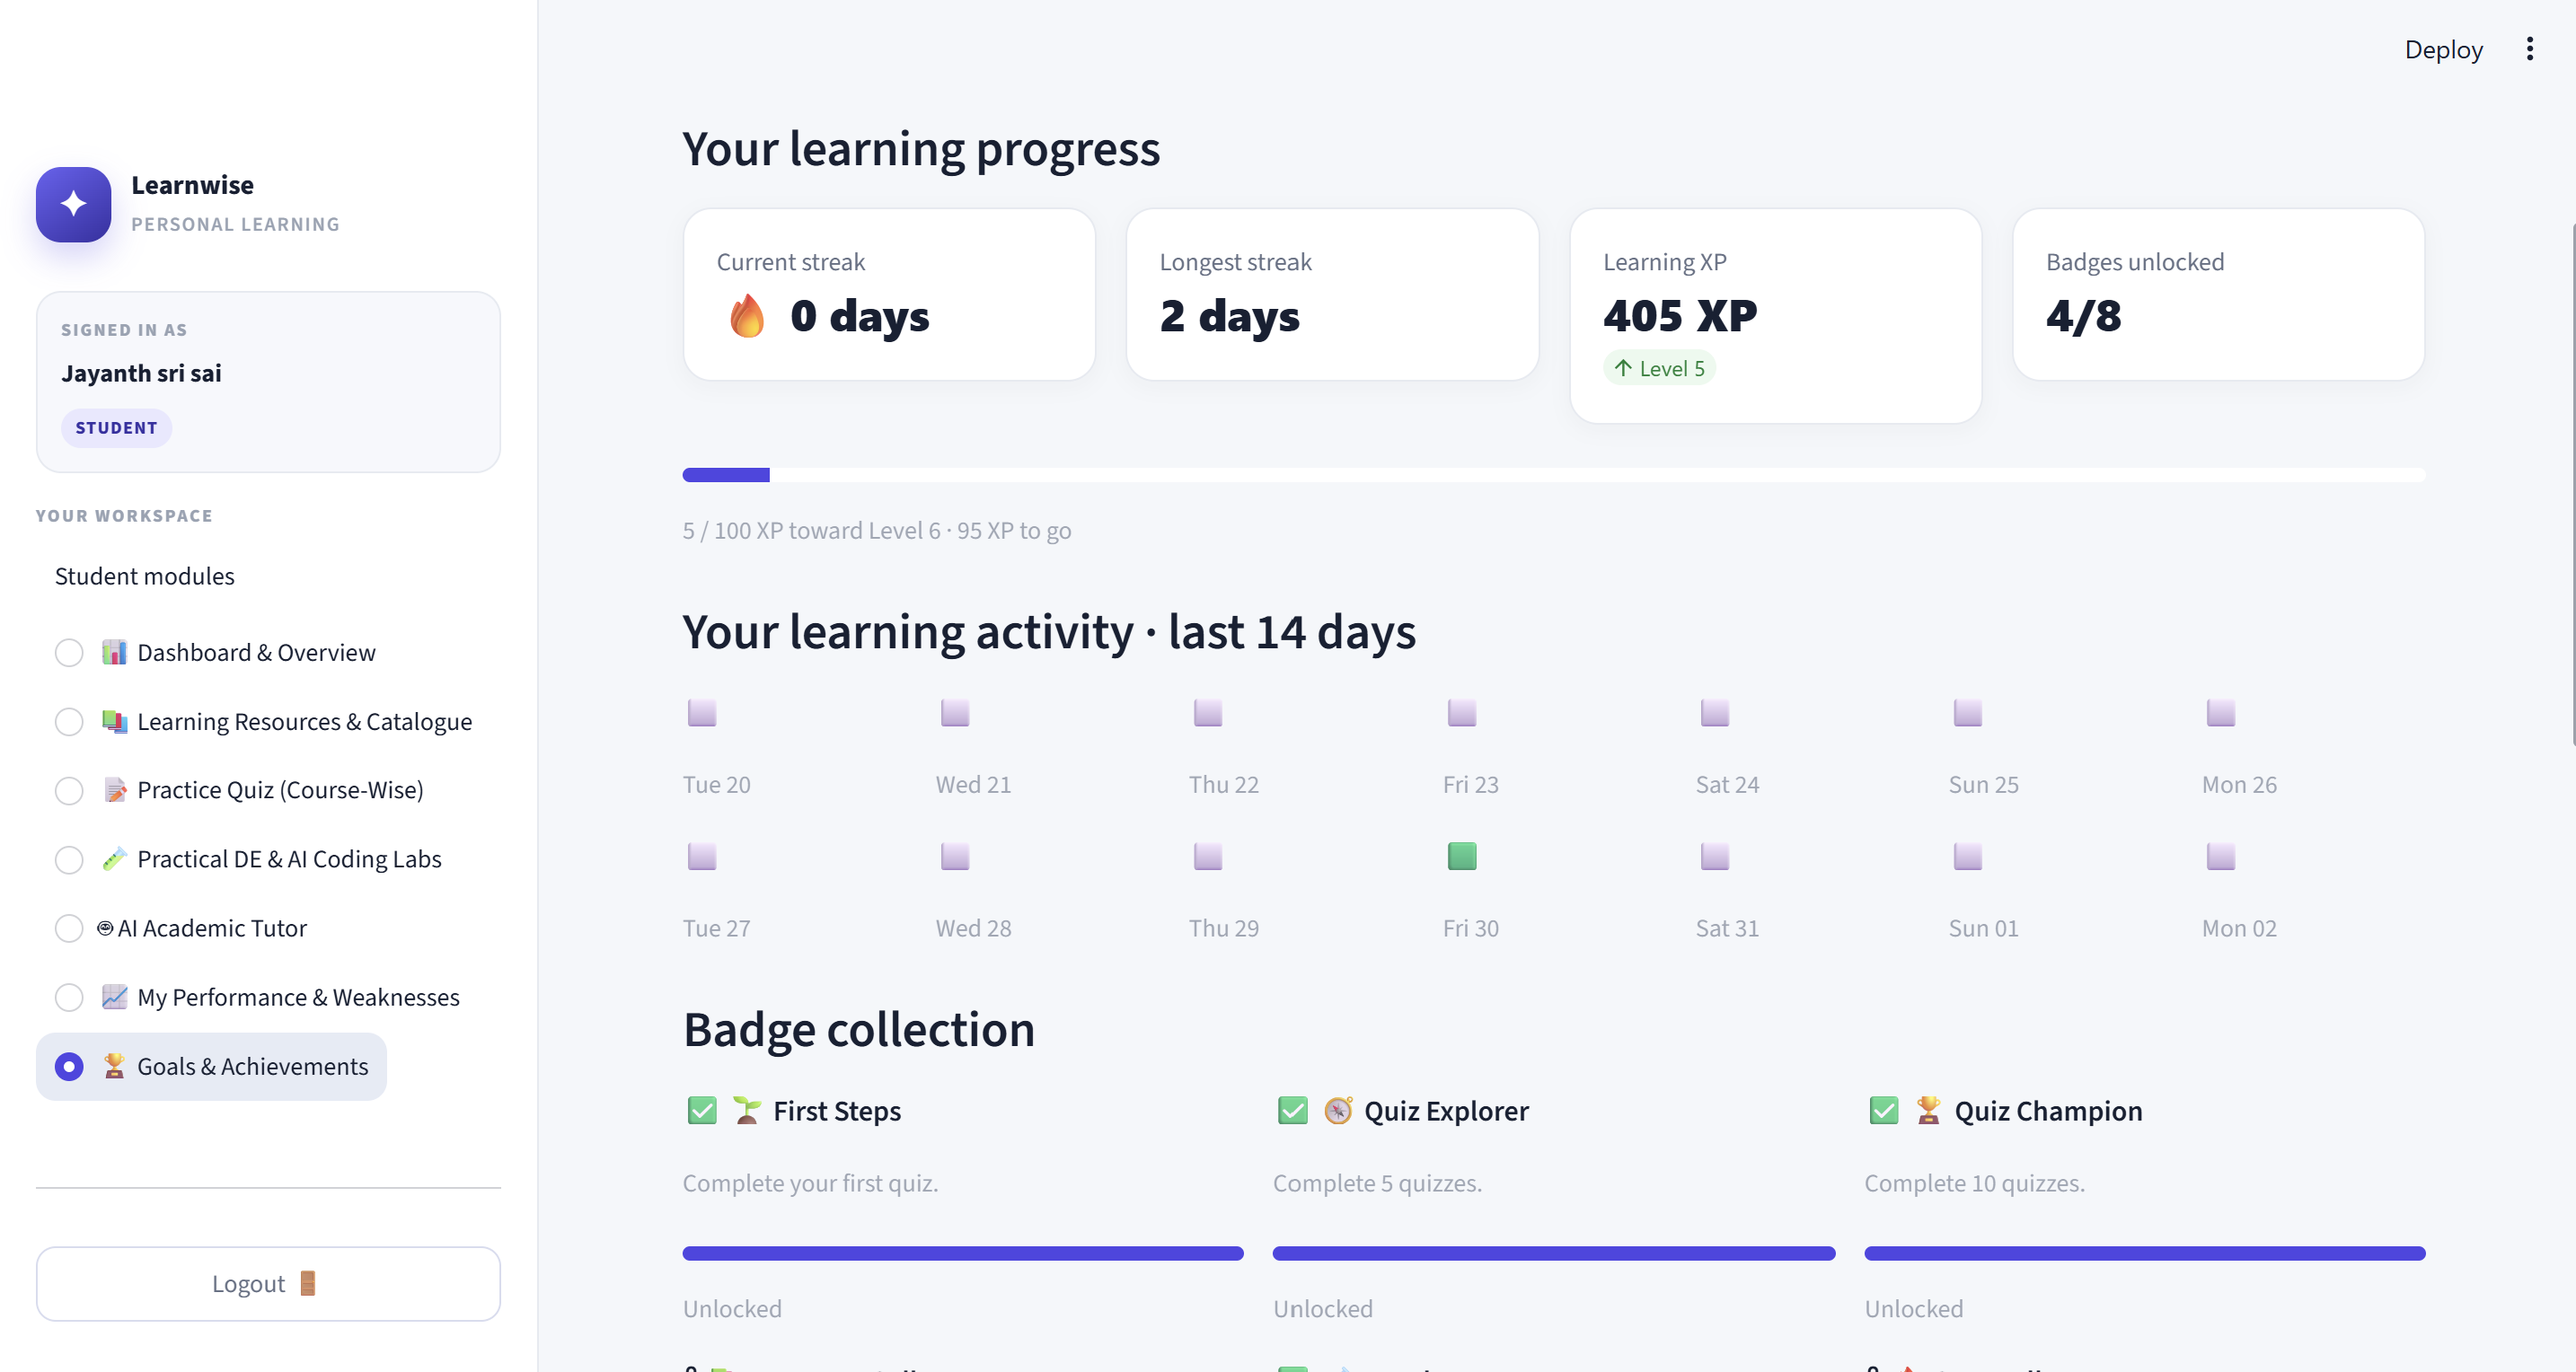
\includegraphics[width=\linewidth,height=1.8in,keepaspectratio]{figures/goals-achievements.png}
\caption{Learning streak, experience points, and achievement badges.}
\label{fig:goals-achievements}
\end{figure}

The screenshots show one account, showing both the state of the application and the screen. The scores shown in the images and the estimated level, streak, XP and skill values shown are not study scores or validated results of the model. Participants and learning-gain comparison are not reported and classroom evaluation is not reported.

\section{Evaluation Status and Future Work}
This manuscript does not include a classroom trial, recruited participants nor measure learning gains, it is a description of implementation. Synthetic test split is not an independent educational validation test set. There is no claim that Learnwise improves achievement, it is not claimed to be able to accurately diagnose student proficiency, or reduce workload for teachers.

There would have to be multiple phases to an empirical evaluation that can be published. First, the classifier needs to be evaluated on a representative and consented data set where the proficiency labels were assigned to classes independently, by precision / recall measures, confusion matrices, and calibration analysis. Second, the teacher or learner relevance ratings and ranking criteria should be used to determine recommendation of the resources and then the outcome should be qualitatively examined for inappropriate resources. Third, if the statement that the program is learning-effective is to be made, it would have to be supported by a pre-registered study with comparison group, appropriate measures of learning, informed consent, and reporting of attrition and subgroups. The accuracy of the quizzes is not to be the only basis of usability or teacher work. These are in line with previous works which reported poor pedagogical assessment in the field of educational recommender systems (ERS) and the diversity of evidence of personalized learning \cite{zhang2020,dasilva2023,tlili2024}.

Others include the use of a single-file database in the local environment as opposed to a multi-institution database, self-reported study time and three categories of learner needs, which are not flexible. The external tutor path is impacted by third party availability and policies. The platform needs to be security reviewed, privacy governed, teacher reviewed, tested with representative learners and platform resource catalogue and question bank need to be reviewed before implementation in class.

\section{Conclusion}
Learnwise is a modular Streamlit app that incorporates learner dashboards, course-based assessment, estimation of learner profiles, resource prioritization, tutor support, and teacher analytics. It describes the data flow and implementation decisions, such as the use of synthetic training labels and deterministic rules for recommendations and alerts, in the paper. The existing system is a software prototype system. Whether or not its value for learning is realisable remains an empirical claim, which should be confirmed through actual learners and assessed measures of learning.



\begin{thebibliography}{20}

\bibitem{zhang2020}
L. Zhang, J. D. Basham, and S. Yang, ``Understanding the implementation of personalized learning: A research synthesis,'' \textit{Educational Research Review}, vol. 31, art. 100339, 2020. doi: \href{https://doi.org/10.1016/j.edurev.2020.100339}{10.1016/j.edurev.2020.100339}.

\bibitem{dasilva2023}
F. L. da Silva, B. K. Slodkowski, K. K. A. da Silva, and S. C. Cazella, ``A systematic literature review on educational recommender systems for teaching and learning: Research trends, limitations and opportunities,'' \textit{Education and Information Technologies}, vol. 28, pp. 3289--3328, 2023. doi: \href{https://doi.org/10.1007/s10639-022-11341-9}{10.1007/s10639-022-11341-9}.

\bibitem{tlili2024}
A. Tlili, S. Salha, H. Wang, R. Huang, J. Rudolph, and W. Ren, ``Does personalization really help in improving learning achievement? A meta-analysis,'' in \textit{Proc. IEEE International Conference on Advanced Learning Technologies (ICALT)}, 2024, pp. 13--17. doi: \href{https://doi.org/10.1109/ICALT61570.2024.00011}{10.1109/ICALT61570.2024.00011}.

\bibitem{brusilovsky2001}
P. Brusilovsky, ``Adaptive hypermedia,'' \textit{User Modeling and User-Adapted Interaction}, vol. 11, nos. 1--2, pp. 87--110, 2001, doi: \href{https://doi.org/10.1023/A:1011143116306}{10.1023/A:1011143116306}.

\bibitem{breiman2001}
L. Breiman, ``Random forests,'' \textit{Machine Learning}, vol. 45, no. 1, pp. 5--32, 2001. doi: \href{https://doi.org/10.1023/A:1010933404324}{10.1023/A:1010933404324}.

\bibitem{corbett1995}
A. T. Corbett and J. R. Anderson, ``Knowledge tracing: Modeling the acquisition of procedural knowledge,'' \textit{User Modeling and User-Adapted Interaction}, vol. 4, no. 4, pp. 253--278, 1995, doi: \href{https://doi.org/10.1007/BF01099821}{10.1007/BF01099821}.

\bibitem{piech2015}
C. Piech, J. Bassen, J. Huang, S. Ganguli, M. Sahami, L. Guibas, and J. Sohl-Dickstein, ``Deep knowledge tracing,'' in \textit{Advances in Neural Information Processing Systems}, vol. 28, 2015, pp. 505--513.

\bibitem{siemens2013}
G. Siemens, ``Learning analytics: The emergence of a discipline,'' \textit{American Behavioral Scientist}, vol. 57, no. 10, pp. 1380--1400, 2013, doi: \href{https://doi.org/10.1177/0002764213498851}{10.1177/0002764213498851}.

\bibitem{romero2010}
C. Romero and S. Ventura, ``Educational data mining: A review of the state of the art,'' \textit{IEEE Transactions on Systems, Man, and Cybernetics, Part C: Applications and Reviews}, vol. 40, no. 6, pp. 601--618, 2010, doi: \href{https://doi.org/10.1109/TSMCC.2010.2053532}{10.1109/TSMCC.2010.2053532}.

\bibitem{verbert2014}
K. Verbert, S. Govaerts, E. Duval, J. L. Santos, F. Van Assche, G. Parra, and J. Klerkx, ``Learning dashboards: An overview and future research opportunities,'' \textit{Personal and Ubiquitous Computing}, vol. 18, no. 6, pp. 1499--1514, 2014, doi: \href{https://doi.org/10.1007/s00779-013-0751-2}{10.1007/s00779-013-0751-2}.

\bibitem{shute2008}
V. J. Shute, ``Focus on formative feedback,'' \textit{Review of Educational Research}, vol. 78, no. 1, pp. 153--189, 2008, doi: \href{https://doi.org/10.3102/0034654307313795}{10.3102/0034654307313795}.

\bibitem{hattie2007}
J. Hattie and H. Timperley, ``The power of feedback,'' \textit{Review of Educational Research}, vol. 77, no. 1, pp. 81--112, 2007, doi: \href{https://doi.org/10.3102/003465430298487}{10.3102/003465430298487}.

\bibitem{nicol2006}
D. J. Nicol and D. Macfarlane-Dick, ``Formative assessment and self-regulated learning: A model and seven principles of good feedback practice,'' \textit{Studies in Higher Education}, vol. 31, no. 2, pp. 199--218, 2006, doi: \href{https://doi.org/10.1080/03075070600572090}{10.1080/03075070600572090}.

\bibitem{zimmerman2002}
B. J. Zimmerman, ``Becoming a self-regulated learner: An overview,'' \textit{Theory Into Practice}, vol. 41, no. 2, pp. 64--70, 2002, doi: \href{https://doi.org/10.1207/S15430421TIP4102_2}{10.1207/S15430421TIP4102\_2}.

\bibitem{koedinger2013}
K. R. Koedinger, E. Brunskill, R. S. J. d. Baker, E. A. McLaughlin, and J. Stamper, ``New potentials for data-driven intelligent tutoring system development and optimization,'' \textit{AI Magazine}, vol. 34, no. 3, pp. 27--41, 2013, doi: \href{https://doi.org/10.1609/aimag.v34i3.2484}{10.1609/aimag.v34i3.2484}.

\bibitem{streamlit}
Streamlit, ``Streamlit documentation.'' [Online]. Available: \url{https://docs.streamlit.io/}. Accessed: Oct. 29, 2026.

\bibitem{sqlite}
SQLite, ``SQLite documentation.'' [Online]. Available: \url{https://www.sqlite.org/docs.html}. Accessed: Oct. 29, 2026.

\bibitem{sklearnrf}
Scikit-learn developers, ``RandomForestClassifier documentation.'' [Online]. Available: \url{https://scikit-learn.org/stable/modules/generated/sklearn.ensemble.RandomForestClassifier.html}. Accessed: Oct. 29, 2026.

\bibitem{pardo2014}
A. Pardo and G. Siemens, ``Ethical and privacy principles for learning analytics,'' \textit{British Journal of Educational Technology}, vol. 45, no. 3, pp. 438--450, 2014, doi: \href{https://doi.org/10.1111/bjet.12152}{10.1111/bjet.12152}.

\bibitem{unesco}
F. Miao and W. Holmes, \textit{Guidance for Generative AI in Education and Research}. Paris, France: UNESCO, 2023. doi: \href{https://doi.org/10.54675/EWZM9535}{10.54675/EWZM9535}.

\end{thebibliography}

\end{document}
f,.//././/,/ k
